\documentclass{beamer}
\usetheme{Madrid}
\usecolortheme{default}
\usepackage{amsmath,amssymb,lmodern}
\usepackage{caption}
\usepackage{listings}
\usepackage{animate}
\usepackage{subcaption}
\usepackage{xcolor}
\usepackage{graphicx} %Loading the package

\graphicspath{{figures/}} %Setting the graphicspath
\title[Machine Learning]
{Treinamento de Machine Learning e Deep Learning}

\subtitle{Do Básico ao Avançado}

\author[Mafalda, Salomão] % (optional, for multiple authors)
{Salomão Machado Mafalda\inst{1}}

\institute[PAVIC] % (optional)
{
  \inst{1}%
  Universidade Federal do Acre\\
  PAVIC

}

\date[2023] % (optional)
{2023}

\logo{
\includegraphics[height=0.8cm]{ente}}

\definecolor{uoftblue}{RGB}{6,41,88}
\setbeamercolor{titlelike}{bg=uoftblue}
\setbeamerfont{title}{series=\bfseries}

\begin{document}

\frame{\titlepage}

\begin{frame}
\frametitle{Agenda}
\tableofcontents
\end{frame}



%==========================================================================================
\section{Perceptron}

\begin{frame}
	\frametitle{Perceptron}
	\begin{figure}
		\centering
		\label{fig:neuron}
		\includegraphics[width=0.4\linewidth]{neuron}
		\caption{Neurônio humano}
	\end{figure}
\end{frame}


%==========================================================================================
\begin{frame}
	\frametitle{Perceptron}
	\begin{figure}
		\centering
		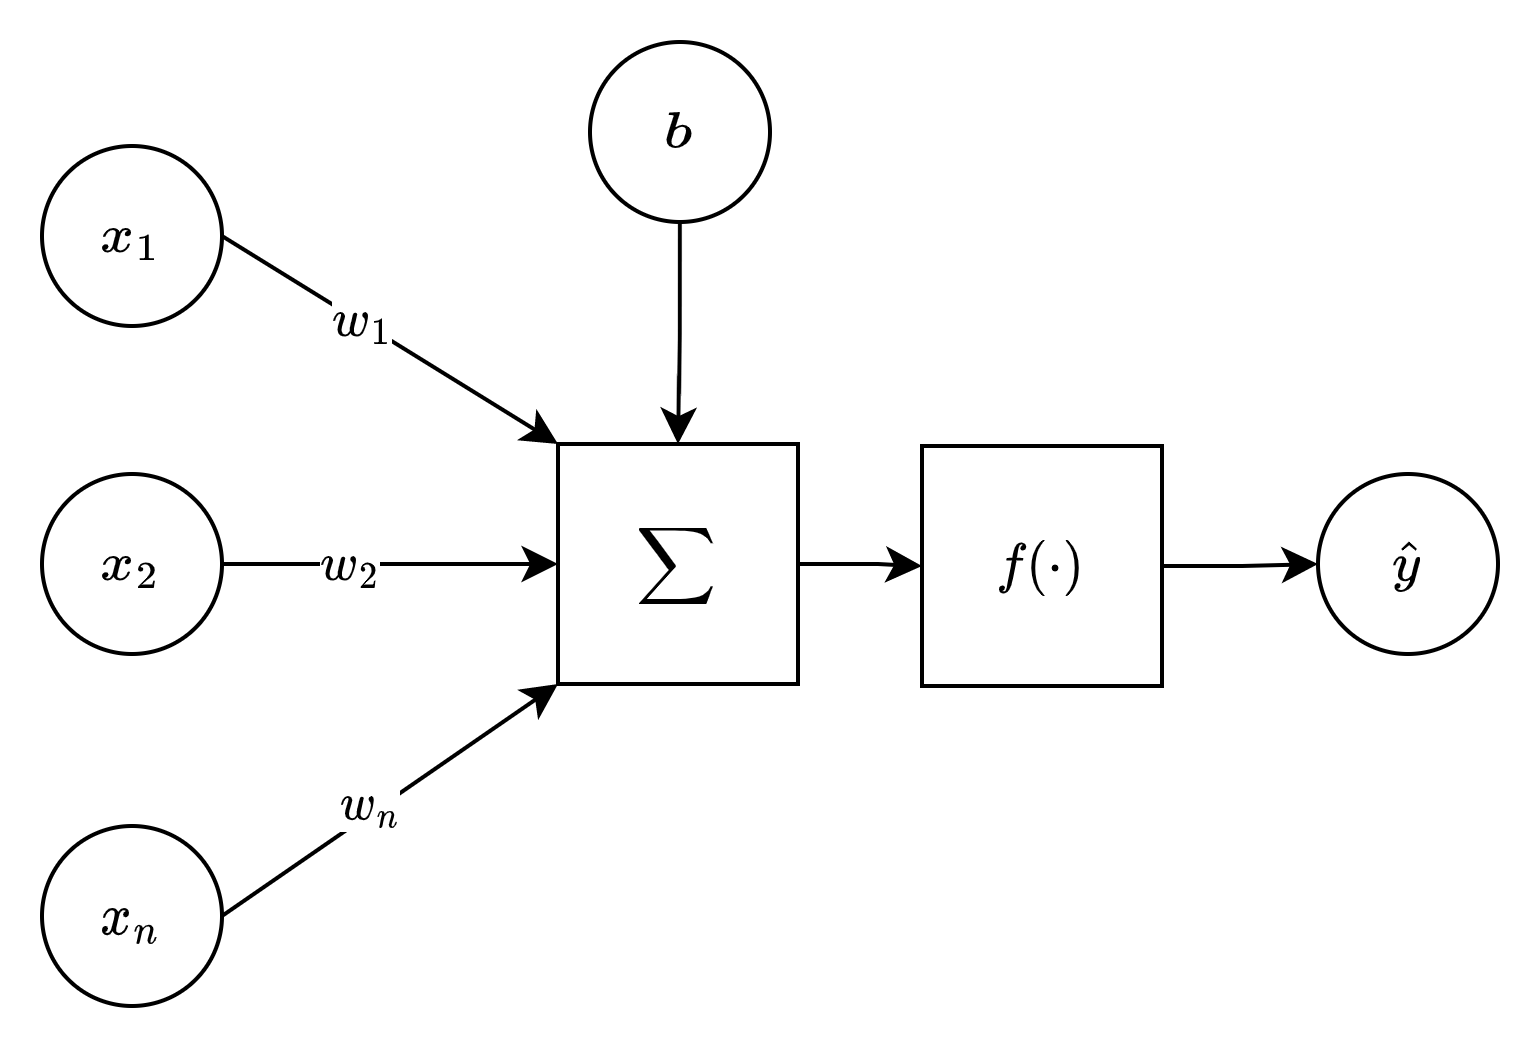
\includegraphics[width=0.4\linewidth]{figures/neuron_ai}
		\caption{Neurônio Artificial}
		\label{fig:neuronai}
	\end{figure}
\end{frame}

%==========================================================================================
\begin{frame}
	\frametitle{Perceptron}
	\begin{figure}
		\centering
		\begin{subfigure}{.45\textwidth}
			\includegraphics[width=1\linewidth]{figures/neuron}
			\caption{Neurônio Humano}
		\end{subfigure}
		\begin{subfigure}{.45\textwidth}
			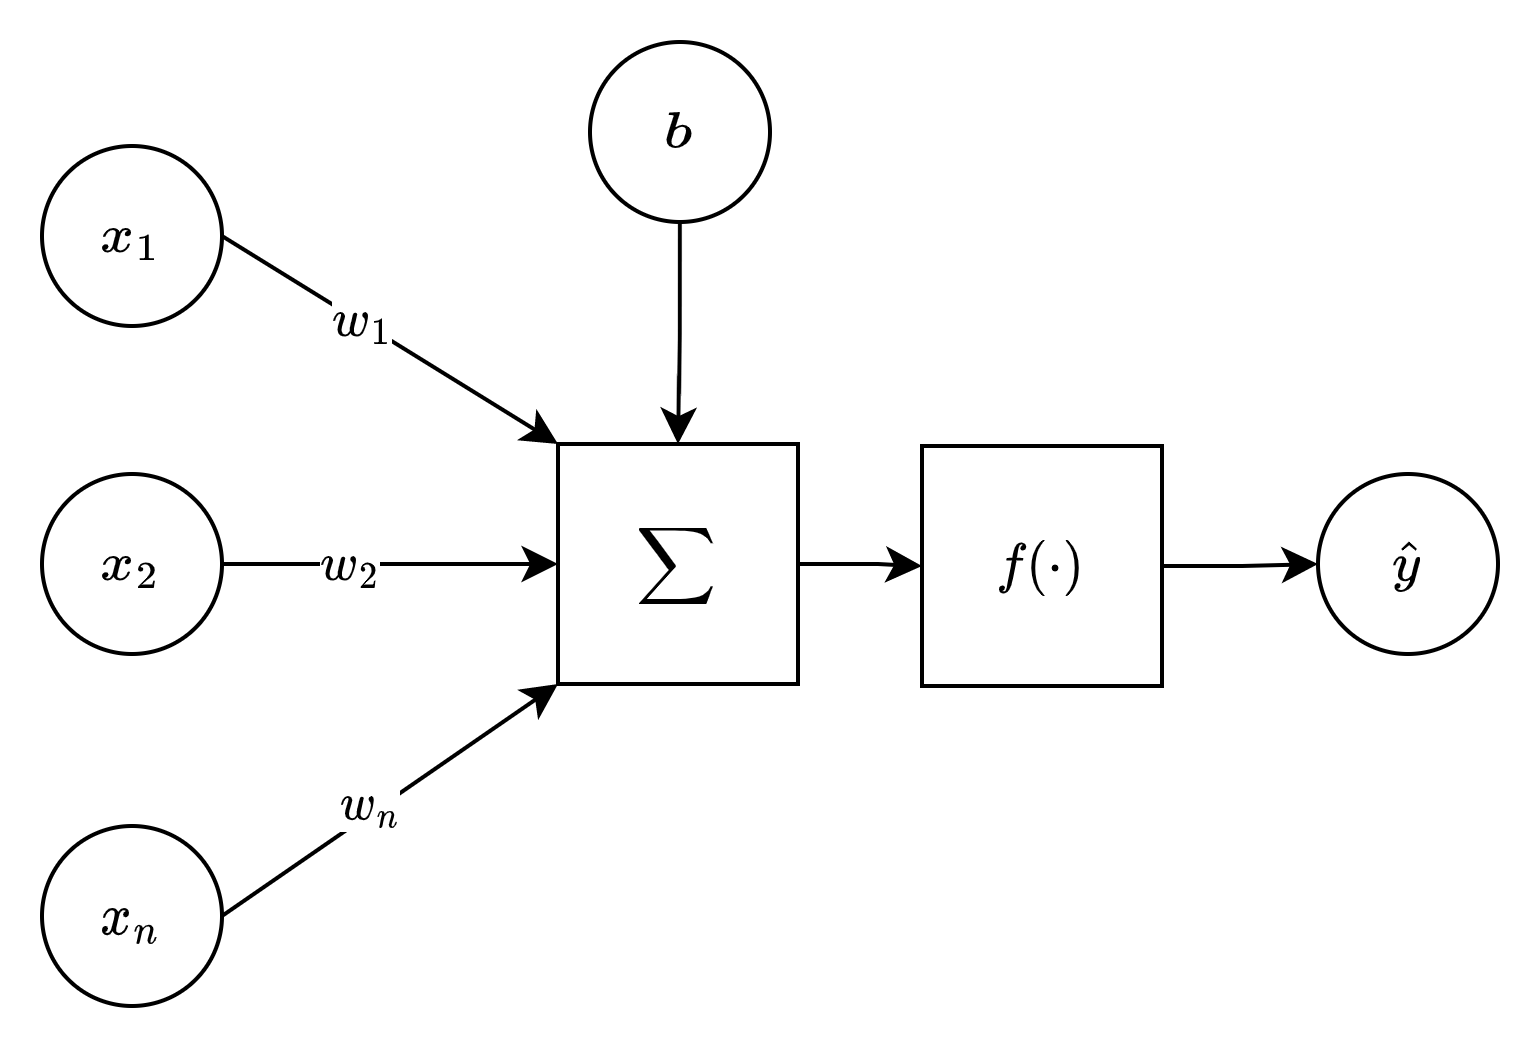
\includegraphics[width=1\linewidth]{figures/neuron_ai}
			\caption{Neurônio Artificial}
		\end{subfigure}
	\end{figure}
\end{frame}
%==========================================================================================
\begin{frame}
	\frametitle{Perceptron}
	\begin{itemize}
		\item Modelo mais básico de NN
		\item Um neurônio
		\item N entradas, Uma saída ŷ
	\end{itemize}
	\begin{figure}
		\centering
		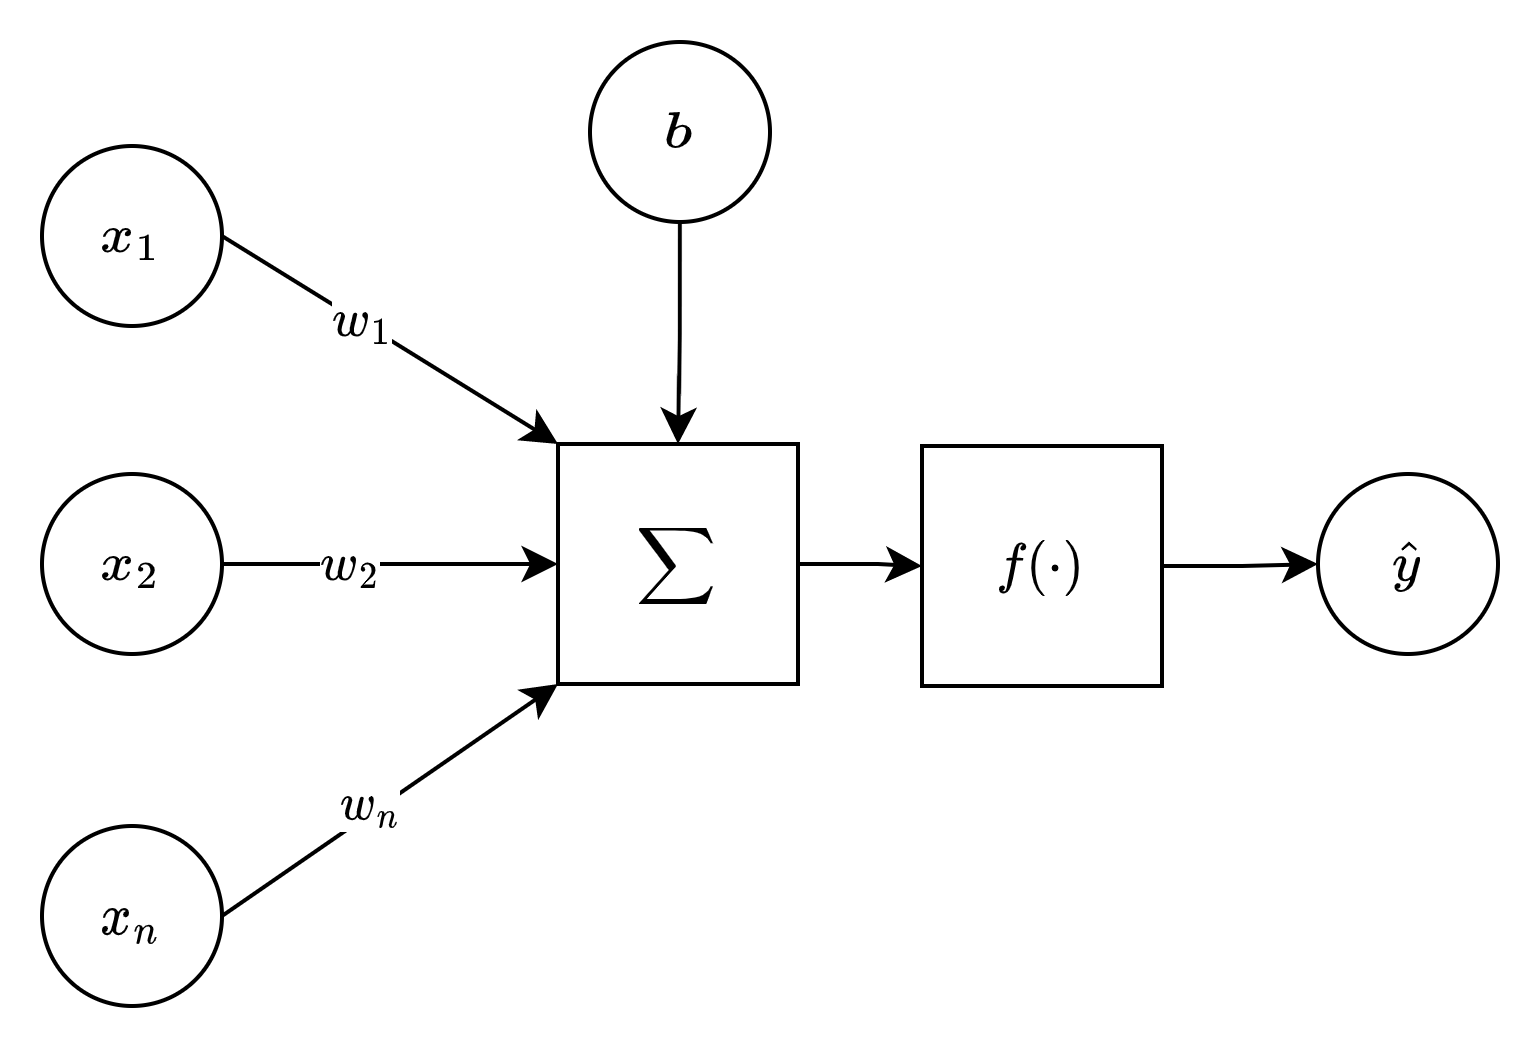
\includegraphics[width=0.4\linewidth]{figures/neuron_ai}
		\caption{Neurônio Artificial}
	\end{figure}

	\begin{gather*}
		\hat{y} = f( \sum_i w_i x_i + b)
	\end{gather*}
\end{frame}
%==========================================================================================
\begin{frame}
	\frametitle{Perceptron}
	\begin{itemize}
		\item Modelo mais básico de NN
		\item Um neurônio
		\item N entradas, Uma saída ŷ
		\item Classificador binário linear
		\item Pode ser usado para Regressão
		\item Perceptron Rule
		\item Aprendizado Online
		\begin{itemize}
			\item Atualiza os pesos por amostra
		\end{itemize}
	\end{itemize}
	\begin{figure}
		\centering
		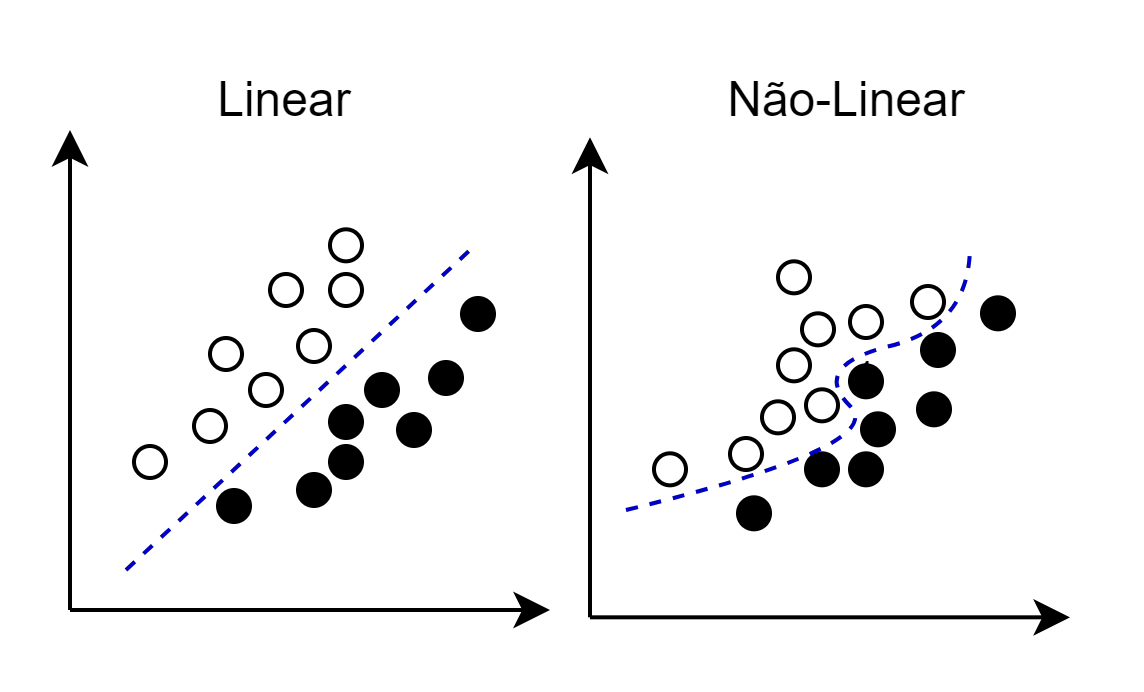
\includegraphics[width=0.6\linewidth]{figures/linear_regression}
	\end{figure}
	
	\begin{gather*}
		\hat{y} = f( \sum_i w_i x_i + b)
	\end{gather*}
\end{frame}
%==========================================================================================
\begin{frame}
	\frametitle{Perceptron}
	\begin{block}{Função de ativação do perceptron}
		$$
		\left\{\begin{matrix}
			0 \; if \; 0 > x
			\\ 
			1 \; if \; x \geq 0
		\end{matrix}\right.$$

		\begin{itemize}
			\item 0 se for negativo
			\item 1 se maior ou igual a 0
		\end{itemize}
	\end{block}
	
	\begin{figure}
		\centering
		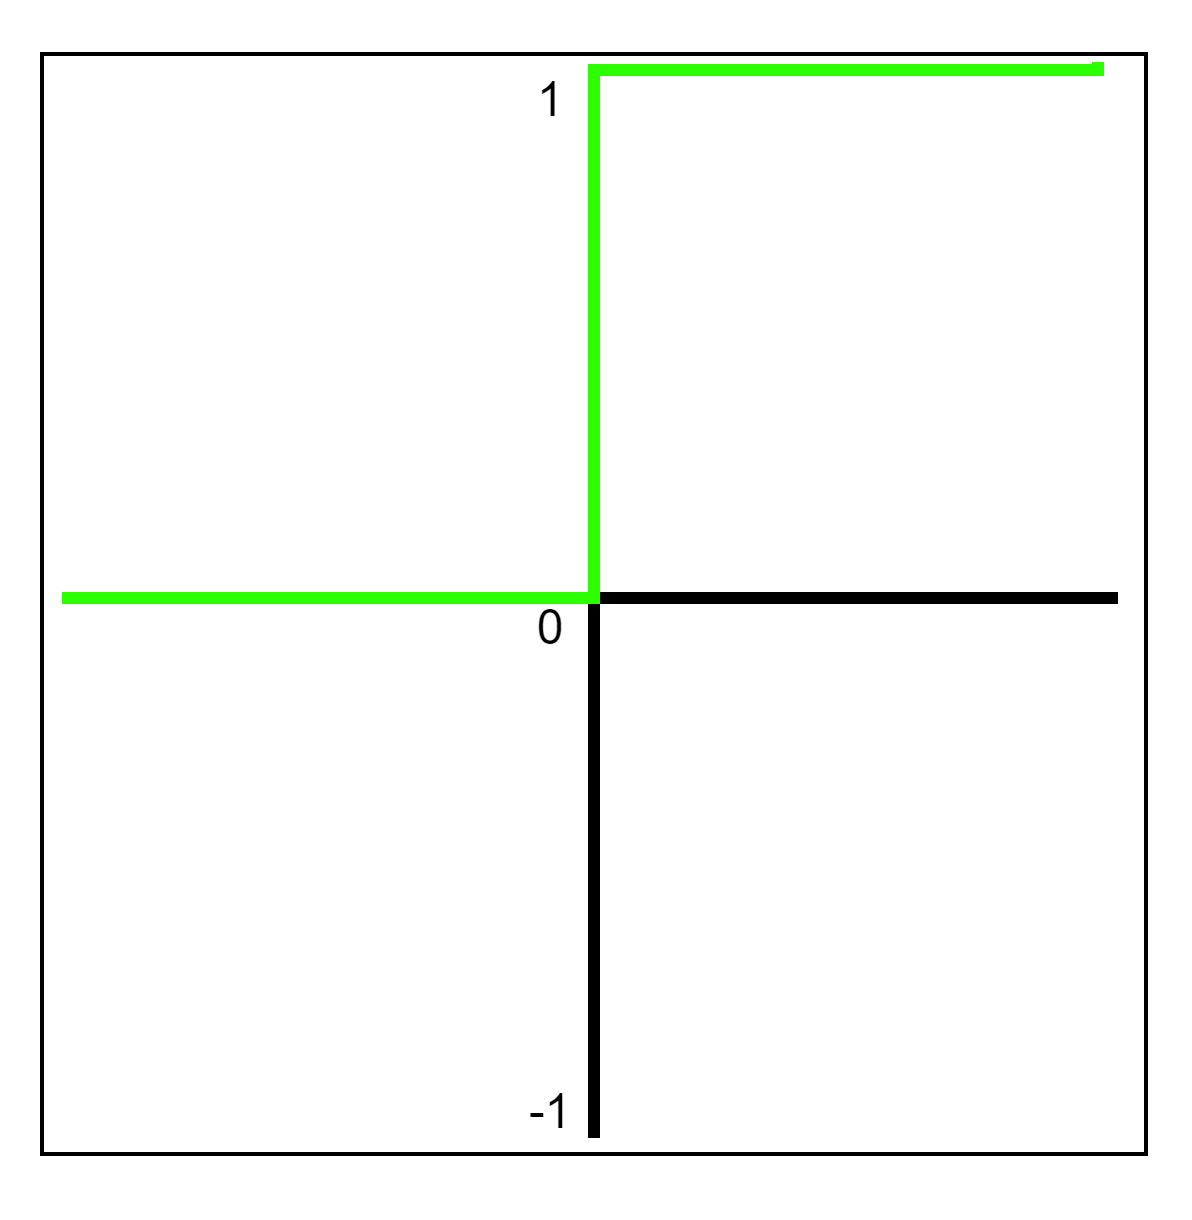
\includegraphics[width=0.35\linewidth]{figures/step_function}
	\end{figure}
\end{frame}
%==========================================================================================

\begin{frame}
	\frametitle{Perceptron}
		\begin{block}{Perceptron Rule}
			O perceptron atualiza seus pesos utilizando a perceptron rule, não com o gradiente
	\end{block}
Atualização dos pesos:
	\begin{gather*}
		w_i = w_i + \lambda*(y_i -  \hat{y}_i)* x_i
	\end{gather*}
	Atualização do \textit{bias}:
	\begin{gather*}
		b_i = b_i + \lambda*(y_i -  \hat{y}_i)
	\end{gather*}
\begin{alertblock}{Observação importante}
``Quando a diferença yi -  ŷi for 0 então não ocorrerá a atualização dos pesos''
\end{alertblock}

\end{frame}
%==========================================================================================

%==========================================================================================
\begin{frame}
	\frametitle{Perceptron}
	\begin{block}{Ponto de partida diferente}
		Com diferentes pontos de partida, o algoritmo encontra quase a mesma solução, embora com diferentes taxas de convergência.
		
		\href{https://github.com/mafaldasalomao/pavic_treinamento_ml/blob/main/Machine_Learning/figures/random_01.gif?raw=true}{\beamergotobutton{Caso 01}} \\
		\href{https://github.com/mafaldasalomao/pavic_treinamento_ml/blob/main/Machine_Learning/figures/random_02.gif?raw=true}{\beamergotobutton{Caso 02}}
	\end{block}
	\begin{block}{Learning Rate - Taxa de aprendizagem}
		\begin{itemize}
			\item LR = 0.01 a velocidade de convergência é muito lenta.
			Quando o cálculo se torna complicado, uma taxa de aprendizado muito baixa afetará a velocidade do algoritmo, mesmo nunca atingindo o destino.
			\item LR = 0.5, o algoritmo se aproxima do alvo muito rapidamente após várias iterações. No entanto, o algoritmo falha ao convergir porque o salto é muito grande, fazendo com que ele fique parado no destino.
		\end{itemize}
		\href{https://github.com/mafaldasalomao/pavic_treinamento_ml/blob/main/Machine_Learning/figures/lr_01.gif}{\beamergotobutton{Caso 01}} \\
		\href{https://github.com/mafaldasalomao/pavic_treinamento_ml/blob/main/Machine_Learning/figures/lr_02.gif}{\beamergotobutton{Caso 02}}
	\end{block}
\end{frame}
%==========================================================================================
\begin{frame}
	\frametitle{Perceptron}
	\begin{block}{Vamos ver na prática}
		Vamos praticar utilizando o notebook 00\_perceptron
	\end{block}
\end{frame}

%==========================================================================================


%==========================================================================================
\section{Adaline}


%==========================================================================================
\begin{frame}
	\frametitle{Adaline}
	\begin{figure}
		\centering
		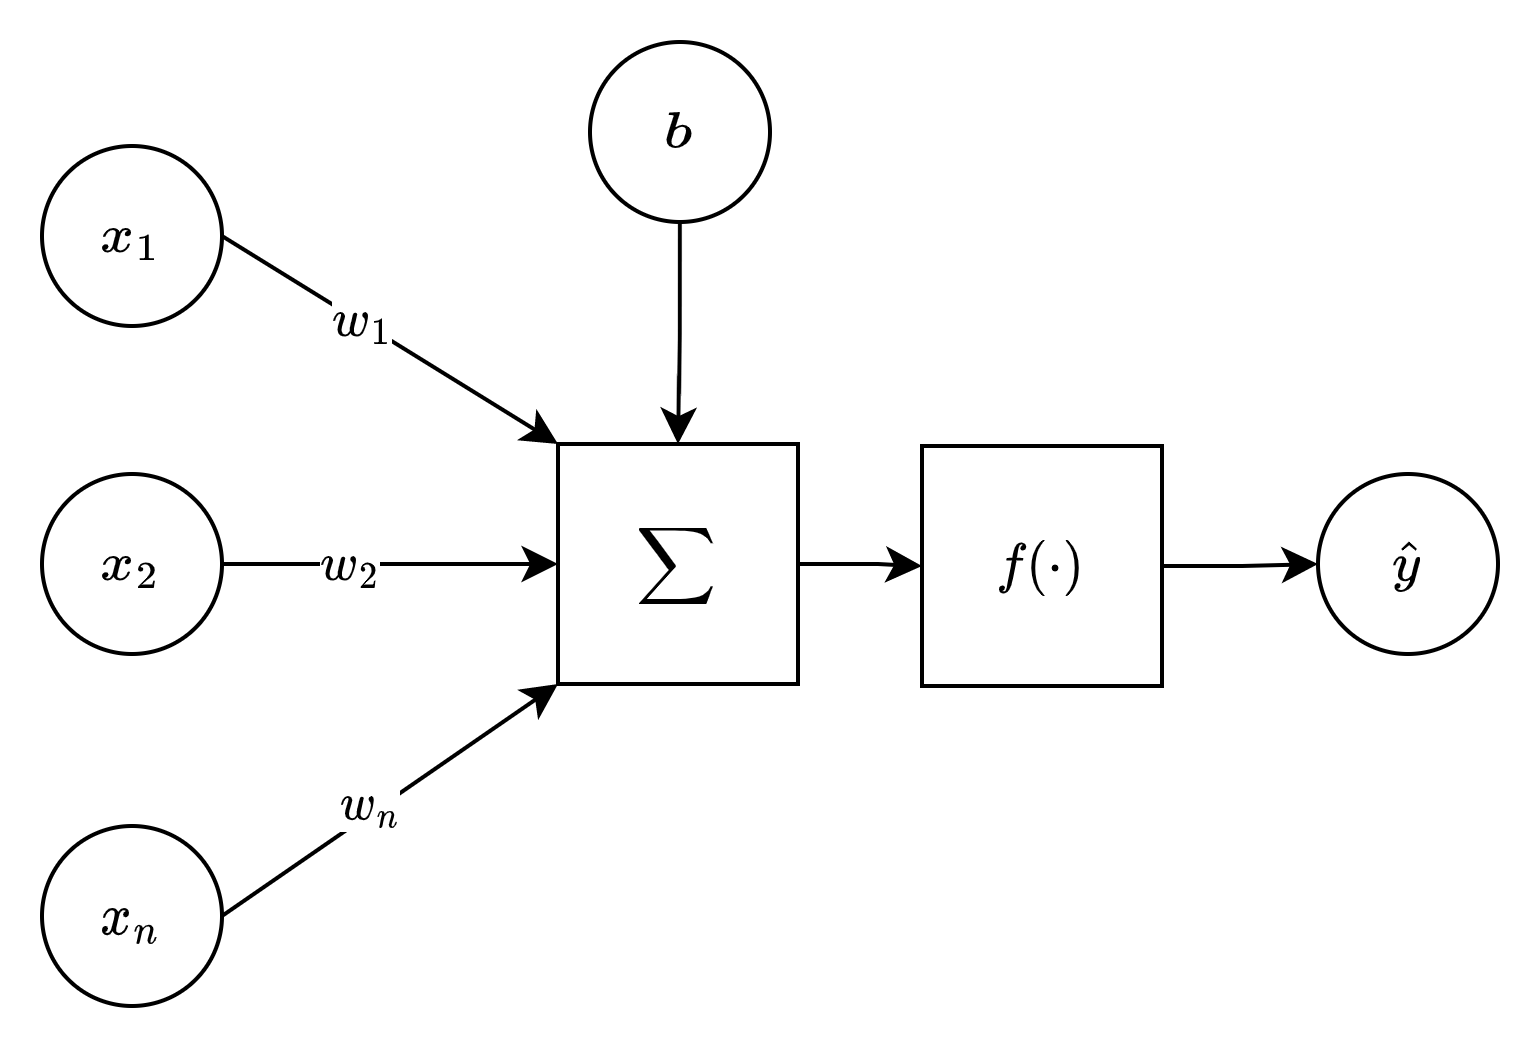
\includegraphics[width=0.4\linewidth]{figures/neuron_ai}
		\caption{Neurônio Artificial}
		\label{fig:neuronai_ada}
	\end{figure}
\end{frame}

%==========================================================================================
%==========================================================================================
%==========================================================================================
\begin{frame}
	\frametitle{Adaline}
	\begin{itemize}
		\item Modelo mais básico de NN
		\item Um neurônio
		\item N entradas, Uma saída ŷ
		\item Classificador binário linear
		\item Pode ser usado para Regressão
		\item Sabe o quanto 'errou'
		\item Aplica-se o gradiente descendente
		\item Aprendizado Online
	\end{itemize}
	
	\begin{gather*}
		\hat{y} = f( \sum_i w_i x_i + b)
	\end{gather*}
\end{frame}
%==========================================================================================
\begin{frame}
	\frametitle{Adaline}
	\begin{block}{Função de ativação do Adaline}
		$$f(x) = x$$
		\begin{itemize}
			\item Possibilita o cálculo da derivada
		\end{itemize}
	\end{block}
	
	\begin{figure}
		\centering
		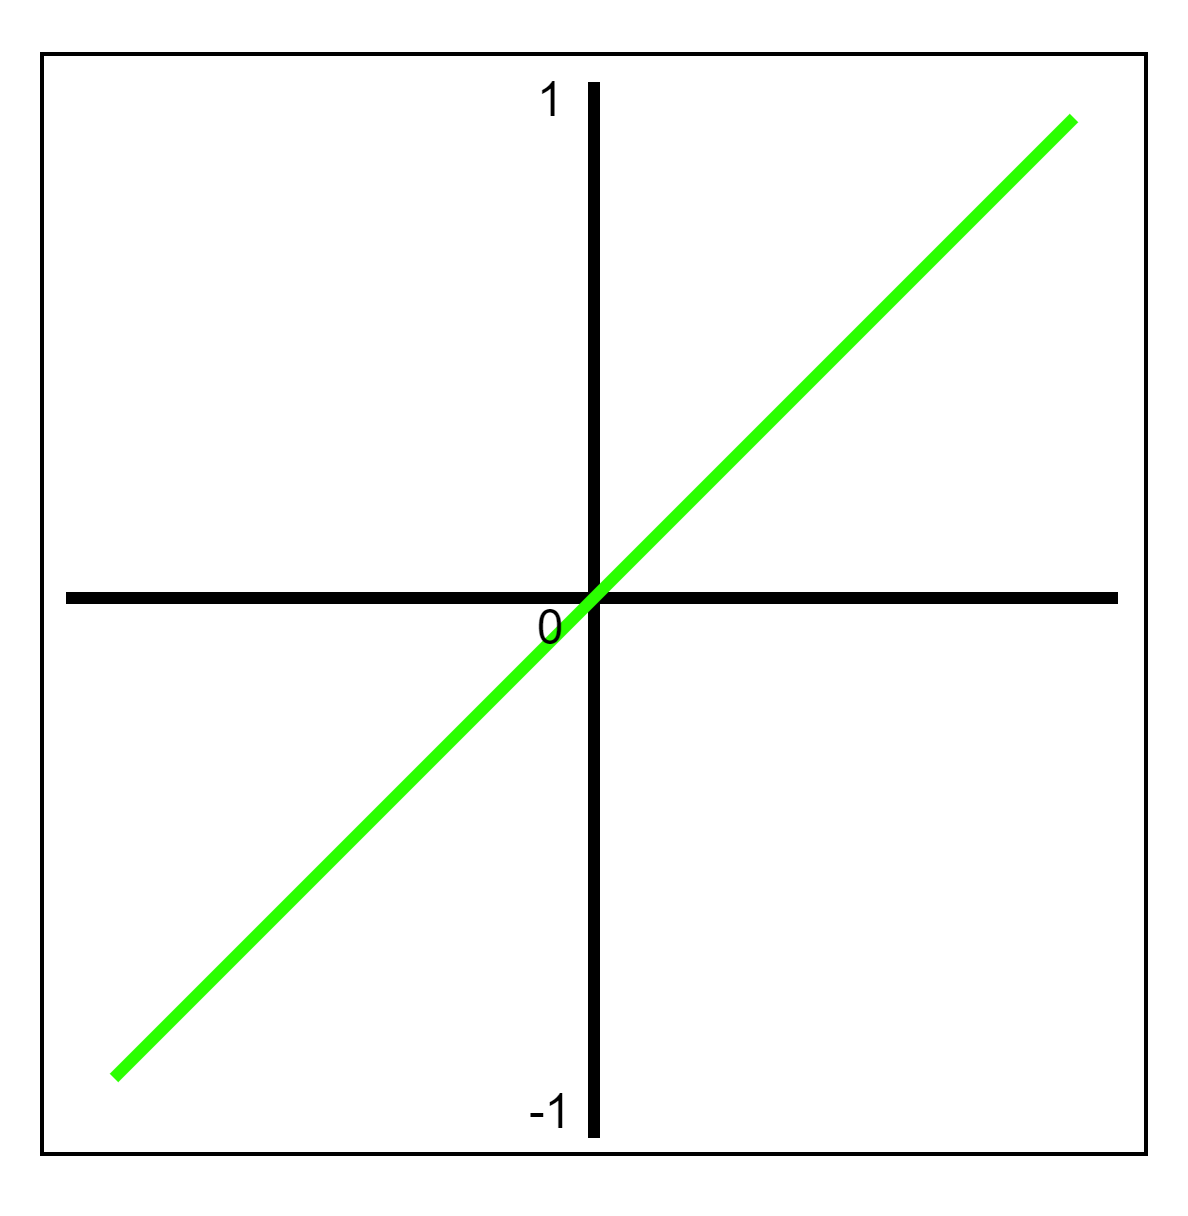
\includegraphics[width=0.35\linewidth]{figures/linear_function}
	\end{figure}

\end{frame}
%==========================================================================================

\begin{frame}
	\frametitle{Adaline vs Perceptron}
	\begin{figure}
		\centering
		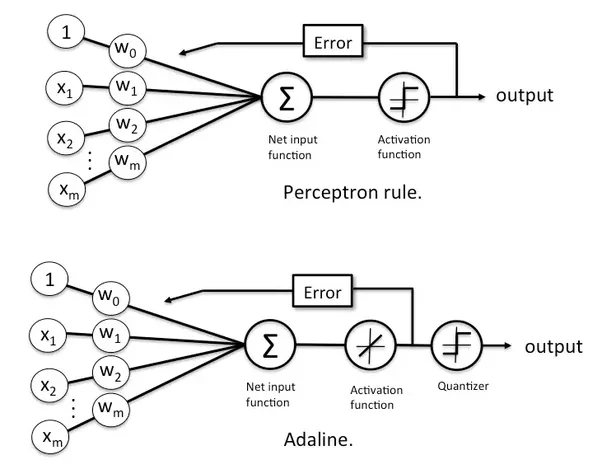
\includegraphics[width=0.7\linewidth]{figures/comparacao_perceptron_adaline}
	\end{figure}
\end{frame}
%==========================================================================================
\begin{frame}
	\frametitle{Adaline vs Perceptron}
	\begin{figure}
		\centering
		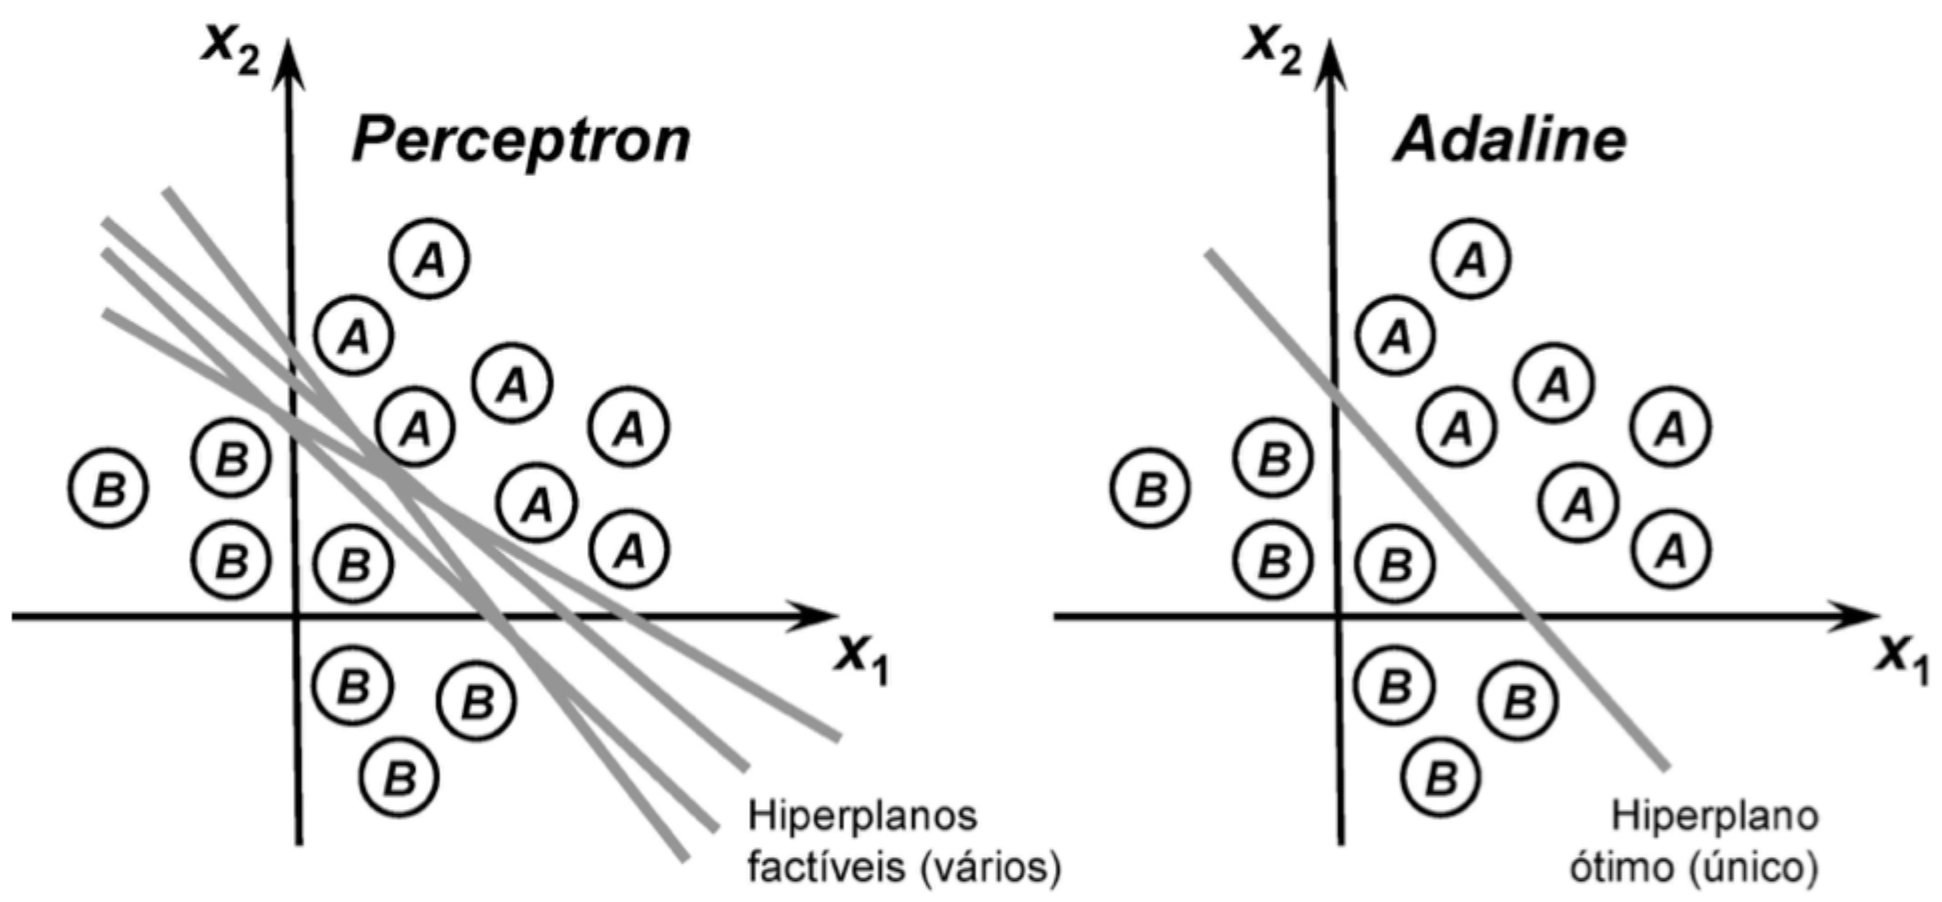
\includegraphics[width=0.9\linewidth]{figures/hiperplanos_perceptron_adaline}
	\end{figure}

\end{frame}
%==========================================================================================
\begin{frame}
	\frametitle{Adaline}
	\begin{block}{Como atualizar os pesos do Adaline}
			\begin{gather*}
			w_i = w_i - \lambda * (y_i - \hat{y}_i) * x_i
		\end{gather*}
	O erro predito será a saída predita menos a saída desejada multiplicados pela entrada (x)
		\begin{gather*}
			J(w) = \frac{1}{2} \sum_{i}^{N} (y_i - \hat{y}_i)^2 \\ 
			\frac{\partial J}{\partial w_i} = \frac{\partial}{\partial w_i} \frac{1}{2} \sum_{i}^{N} (y_i - \hat{y}_i)^2 = \frac{1}{2} \sum_{i}^{N}\frac{\partial}{\partial w_i} (y_i - \hat{y}_i)^2  \\
			= \sum_{i}^{N}(y_i - \hat{y}_i)\frac{\partial}{\partial w_i} (y_i - \hat{y}_i) = \sum_{i}^{N}(y_i - \hat{y}_i) (x_i) \to \frac{\partial J}{\vec{w}} = - (\vec{y}- \vec{\hat{y}})\vec{x}
		\end{gather*}
	\end{block}

		
\end{frame}
%==========================================================================================
\begin{frame}
	\frametitle{Adaline}
	\begin{block}{Vamos ver na prática}
		Vamos praticar utilizando o notebook 01\_adaline
	\end{block}
\end{frame}

%==========================================================================================

\section{Neurônio Sigmoide}


%==========================================================================================
\begin{frame}
	\frametitle{Neurônio Sigmoide}
	\begin{figure}
		\centering
		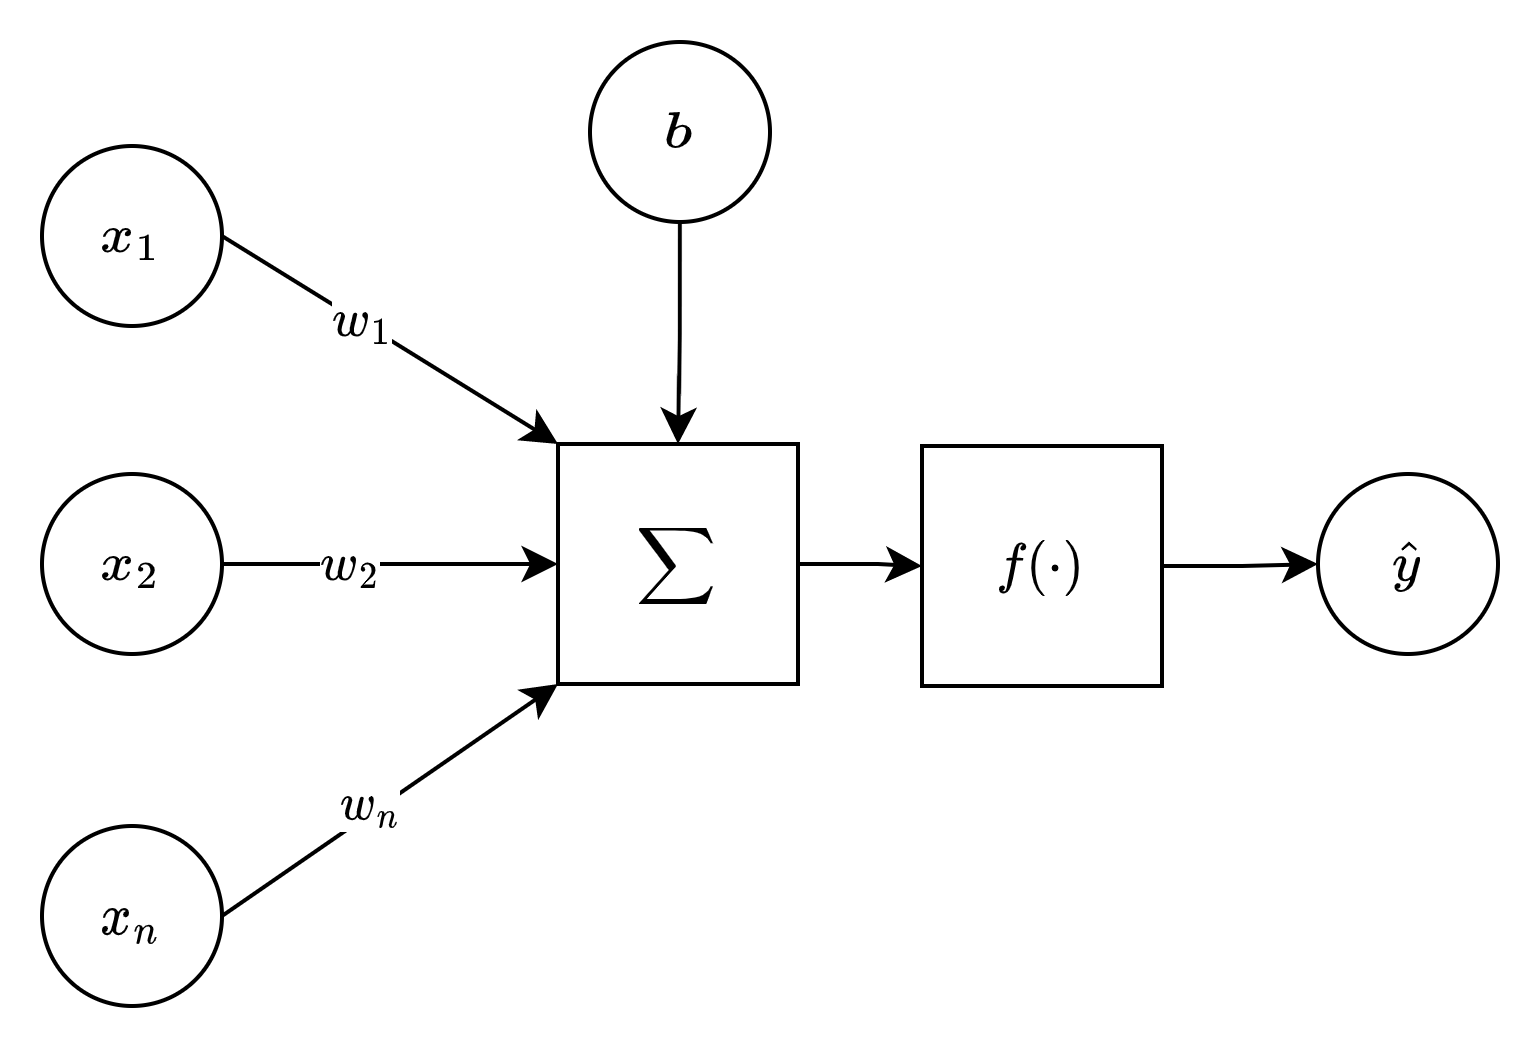
\includegraphics[width=0.4\linewidth]{figures/neuron_ai}
		\caption{Neurônio Artificial}
		\label{fig:neuronai_sig}
	\end{figure}
\end{frame}

%==========================================================================================
%==========================================================================================
%==========================================================================================
\begin{frame}
	\frametitle{Neurônio Sigmoide}
	\begin{itemize}
		\item Modelo mais básico de NN
		\item Um neurônio
		\item N entradas, Uma saída ŷ
		\item Custo: Entropia Cruzada
		\item Classificação binária não-linear
		\item Pequenas alterações nos parâmetros geram pequenas alterações nas saídas
		\item Sabe o quanto 'errou'
		\item Aplica-se o gradiente descendente
	\end{itemize}
	
	\begin{gather*}
		\hat{y} = f( \sum_i w_i x_i + b)
	\end{gather*}
\end{frame}
%==========================================================================================
\begin{frame}
	\frametitle{Neurônio Sigmoide}
	\begin{block}{Função de ativação do Neurônio Sigmoide}
		$$f(x) = \frac{1}{1-e^{-x}}$$
		\begin{itemize}
			\item Possibilita o cálculo da derivada em todos pontos
			\item Aplicado em problemas de regressão logística
		\end{itemize}
	\end{block}
	
\begin{figure}
	\centering
	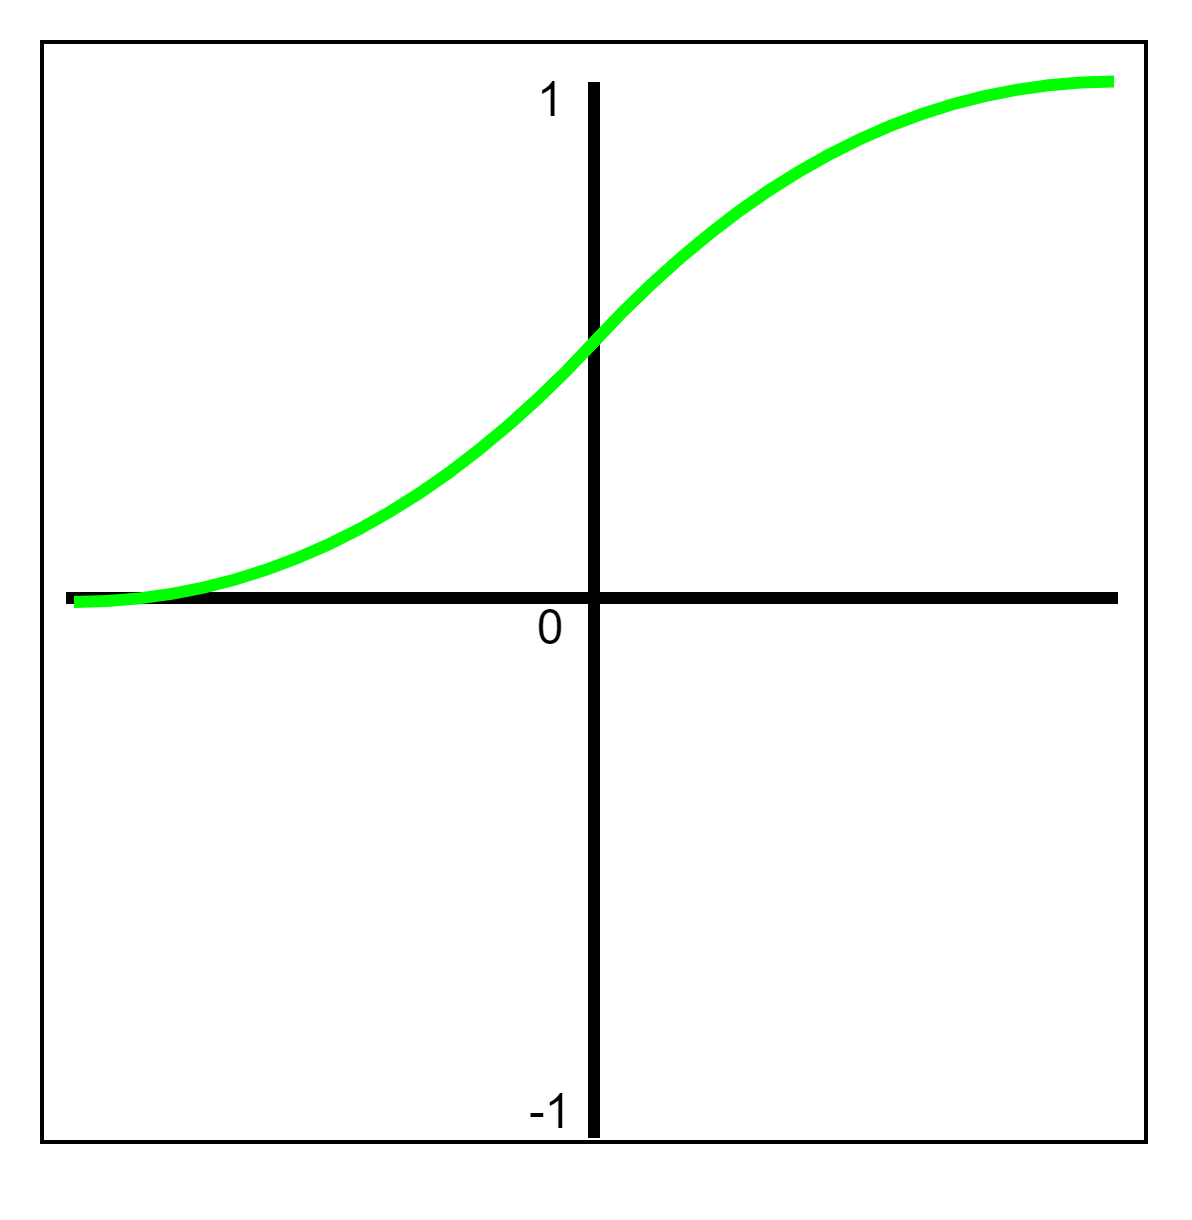
\includegraphics[width=0.35\linewidth]{figures/sigmoid_function}
\end{figure}

	
\end{frame}
%==========================================================================================

\begin{frame}
	\frametitle{Neurônio Sigmoide}
	\begin{block}{Entropia Cruzada}
		$p_j$ é o valor a ser predito e $t_j$ é o valor predito
		\begin{gather*}
			L = - \frac{1}{N} \left [ \sum_{j=1}^{N} [t_j log(p_j) + (1-t_j)log(1-p_j)] \right ] 
		\end{gather*}
	\end{block}
\end{frame}
%==========================================================================================

\begin{frame}
	\frametitle{Neurônio Sigmoide}
	Vamos tomar:
	% Please add the following required packages to your document preamble:
	% \usepackage[table,xcdraw]{xcolor}
	% If you use beamer only pass "xcolor=table" option, i.e. \documentclass[xcolor=table]{beamer}
	\begin{table}[]
		\begin{tabular}{|l|l|l|l|}
			\hline
			$p_j$ & $t_j$ & Erro  & $L$ \\ \hline
			0  & 0  & 0 - 0 = 0  & \textcolor{green}{0}  \\ \hline
			0  & 1  & 0 - 1 = -1 & $\infty$ \\ \hline
			1  & 0  & 1 - 0 = 1  & $\infty$ \\ \hline
			1  & 1  & 1 - 1 = 0  & 0 \\ \hline
		\end{tabular}
	\end{table}
	\begin{block}{Entropia Cruzada}
		Para entrada $0, 0$ e saída predita $\textcolor{red}{0}$ e a saída desejada for $\textcolor{blue}{0}$
		\begin{gather*}
			L = - \frac{1}{N} \left [ \sum_{j=1}^{N} [\textcolor{red}{0} log(\textcolor{blue}{0} ) + (1-\textcolor{red}{0})log(1-\textcolor{blue}{0} )] \right ] 
		\end{gather*}
	\end{block}
\end{frame}
%==========================================================================================
\begin{frame}
	\frametitle{Neurônio Sigmoide}
	Vamos tomar:
	% Please add the following required packages to your document preamble:
	% \usepackage[table,xcdraw]{xcolor}
	% If you use beamer only pass "xcolor=table" option, i.e. \documentclass[xcolor=table]{beamer}
	\begin{table}[]
		\begin{tabular}{|l|l|l|l|}
			\hline
			$p_j$ & $t_j$ & Erro  & $L$ \\ \hline
			0  & 0  & 0 - 0 = 0  & \textcolor{green}{0}  \\ \hline
			0  & 1  & 0 - 1 = -1 & \textcolor{red}{$\infty$} \\ \hline
			1  & 0  & 1 - 0 = 1  & $\infty$ \\ \hline
			1  & 1  & 1 - 1 = 0  & 0 \\ \hline
		\end{tabular}
	\end{table}
	\begin{block}{Entropia Cruzada}
		Para entrada $0, 1$ e saída predita $\textcolor{red}{0}$ e a saída desejada for $\textcolor{blue}{1}$
		\begin{gather*}
			L = - \frac{1}{N} \left [ \sum_{j=1}^{N} [\textcolor{red}{0} log(\textcolor{blue}{1} ) + (1-\textcolor{red}{0})log(1-\textcolor{blue}{1} )] \right ] 
		\end{gather*}
	\end{block}
\end{frame}
%==========================================================================================
\begin{frame}
	\frametitle{Neurônio Sigmoide}
	Vamos tomar:
	\begin{table}[]
	\begin{tabular}{|l|l|l|l|}
		\hline
		$p_j$ & $t_j$ & Erro  & $L$ \\ \hline
		0  & 0  & 0 - 0 = 0  & \textcolor{green}{0}  \\ \hline
		0  & 1  & 0 - 1 = -1 & \textcolor{red}{$\infty$} \\ \hline
		1  & 0  & 1 - 0 = 1  & \textcolor{red}{$\infty$} \\ \hline
		1  & 1  & 1 - 1 = 0  & 0 \\ \hline
	\end{tabular}
\end{table}
\begin{block}{Entropia Cruzada}
	Para entrada $1, 0$ e saída predita $\textcolor{red}{1}$ e a saída desejada for $\textcolor{blue}{0}$
	\begin{gather*}
		L = - \frac{1}{N} \left [ \sum_{j=1}^{N} [\textcolor{red}{1} log(\textcolor{blue}{0} ) + (1-\textcolor{red}{1})log(1-\textcolor{blue}{0} )] \right ] 
	\end{gather*}
\end{block}
\end{frame}
%==========================================================================================
\begin{frame}
	\frametitle{Neurônio Sigmoide}
	Vamos tomar:
	\begin{table}[]
		\begin{tabular}{|l|l|l|l|}
			\hline
			$p_j$ & $t_j$ & Erro  & $L$ \\ \hline
			0  & 0  & 0 - 0 = 0  & \textcolor{green}{0}  \\ \hline
			0  & 1  & 0 - 1 = -1 & \textcolor{red}{$\infty$} \\ \hline
			1  & 0  & 1 - 0 = 1  & \textcolor{red}{$\infty$} \\ \hline
			1  & 1  & 1 - 1 = 0  & \textcolor{green}{0} \\ \hline
		\end{tabular}
	\end{table}
	\begin{block}{Entropia Cruzada}
		Para entrada $1, 1$ e saída predita $\textcolor{red}{1}$ e a saída desejada for $\textcolor{blue}{1}$
		\begin{gather*}
			L = - \frac{1}{N} \left [ \sum_{j=1}^{N} [\textcolor{red}{1} log(\textcolor{blue}{1} ) + (1-\textcolor{red}{1})log(1-\textcolor{blue}{1} )] \right ] 
		\end{gather*}
	\end{block}
\end{frame}

%==========================================================================================
\begin{frame}
	\frametitle{Neurônio Sigmoide}
	\begin{block}{Vamos ver na prática}
		Vamos praticar utilizando o notebook 02\_neuronio\_sigmoid
	\end{block}
\end{frame}

%==========================================================================================
\section{Funções de Ativação}
\begin{frame}
	\frametitle{Funções de Ativação}
	\begin{itemize}
		\item Localizada a saída de cada neurônio
		\item Usada para mapear entradas em novas saídas
		\item Pode alterar o range ex: $[-100 \; 100]$ para $[1 \; 0]$
	\end{itemize}
	\begin{figure}
		\centering
		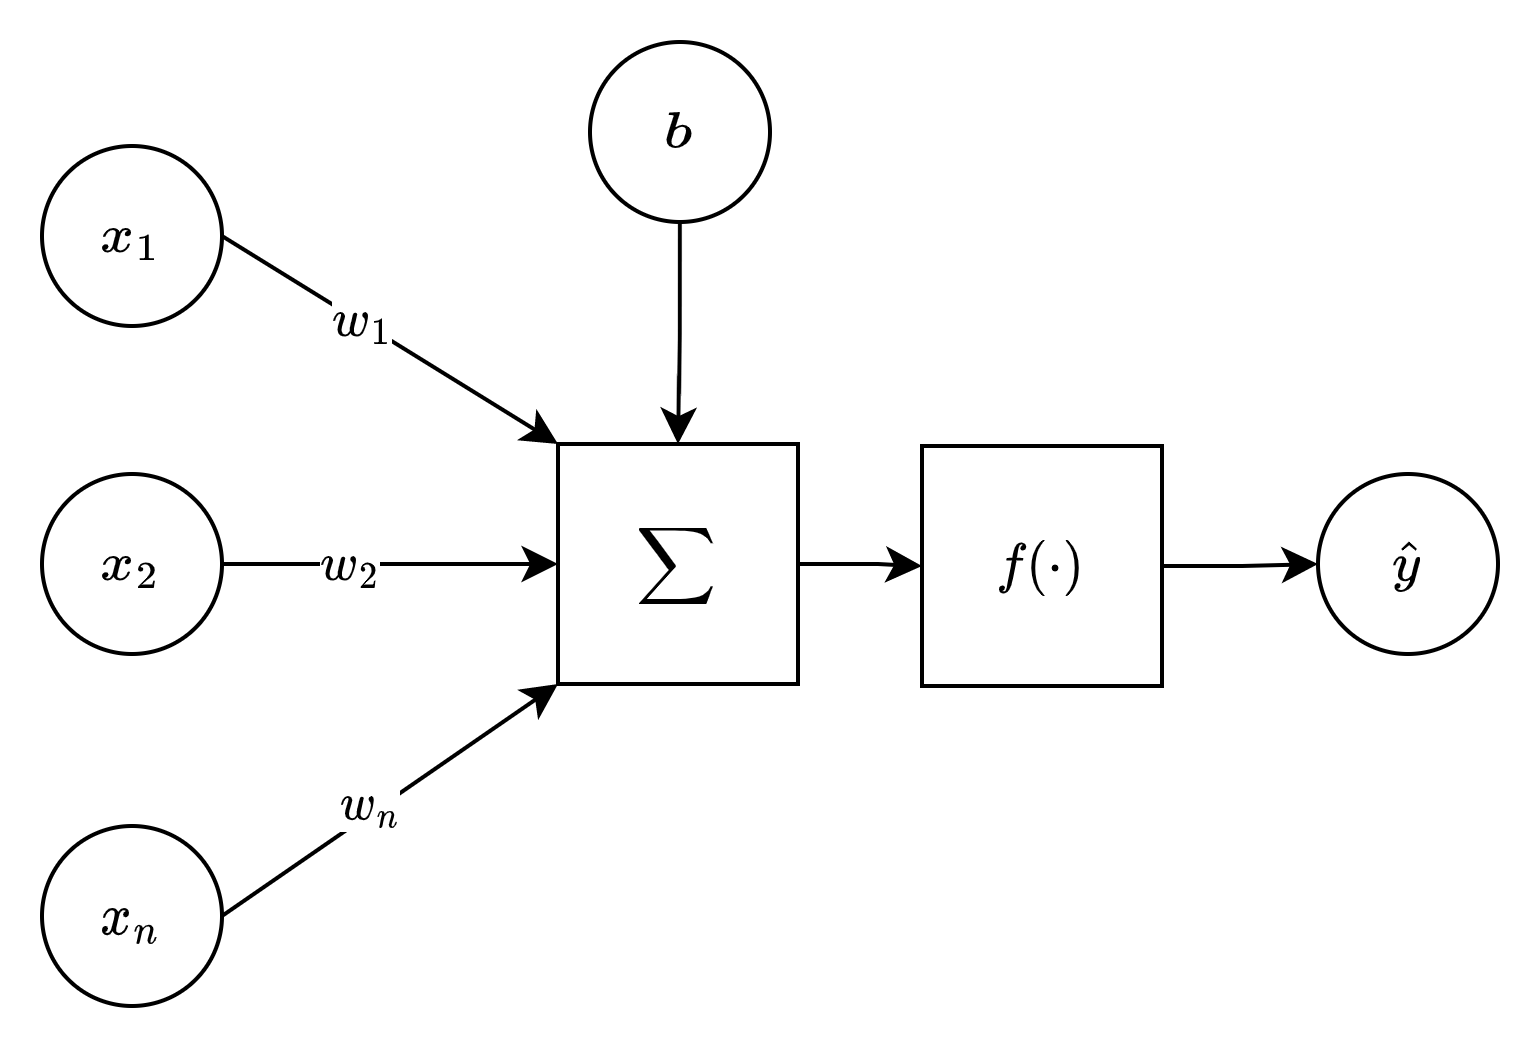
\includegraphics[width=0.4\linewidth]{figures/neuron_ai}
		\caption{Neurônio Artificial}
	\end{figure}
	
	\begin{gather*}
		\hat{y} = f( \sum_i w_i x_i + b)
	\end{gather*}
\end{frame}

%==========================================================================================
\begin{frame}
	\frametitle{Funções de Ativação}
	\begin{block}{Linear}
		\begin{itemize}
			\item $y \in [- \infty, + \infty]$
			\item Função de ativação simples
			\item Comumente usada em regressão
			\item Baixa complexidade
			\item Baixo poder de aprendizagem
		\end{itemize}
	Função:
			$$f(x) = x$$
	Derivada: 	$$\frac{\partial y}{\partial x} = 1$$
	
	\end{block}
\end{frame}

%==========================================================================================
\begin{frame}
	\frametitle{Funções de Ativação}
	\begin{alertblock}{Atenção}
		Note este caso: Porque construir modelos apenas com Lineares? \\
		input:	``10 → 100 → 200 → 10'' \\
		pesos:	``10 → 2 → 00.5 = 10 x 10 = 10'' \\
		Podemos substituir todos pesos por um só
	\end{alertblock}
	\begin{figure}
		\centering
		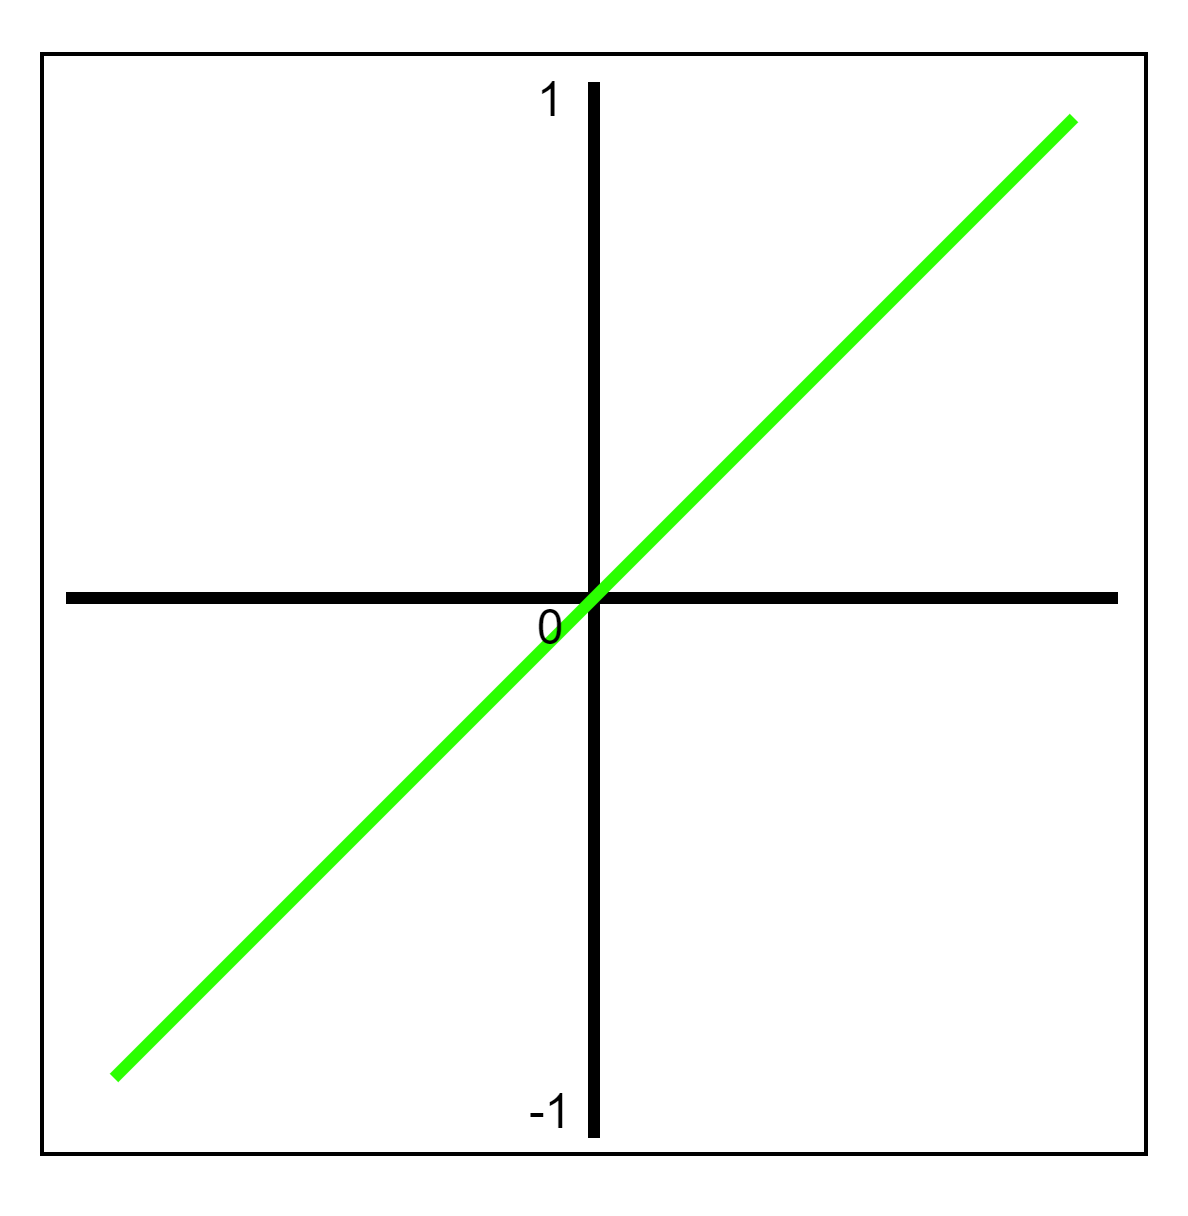
\includegraphics[width=0.4\linewidth]{figures/linear_function.png}
	\end{figure}
\end{frame}
%==========================================================================================
\begin{frame}
	\frametitle{Funções de Ativação}
	\begin{block}{Sigmoid}
		\begin{itemize}
			\item $y \in [0, + 1]$
			\item Regressão Logística
			\item Geralmente interpretada como probabilidade
			\item Saída não centrada em $0$
			\item Satura os gradientes
			\item Não indicada para camadas ocultas
			\item Converge lentamente
		\end{itemize}
		Função:
		$$f(x) = \frac{1}{1-e^{-x}}$$
		Derivada: 	$$\frac{\partial y}{\partial x} = y(1-y)$$
	\end{block}
\end{frame}
%==========================================================================================
\begin{frame}
	\frametitle{Funções de Ativação}
\begin{figure}
	\centering
	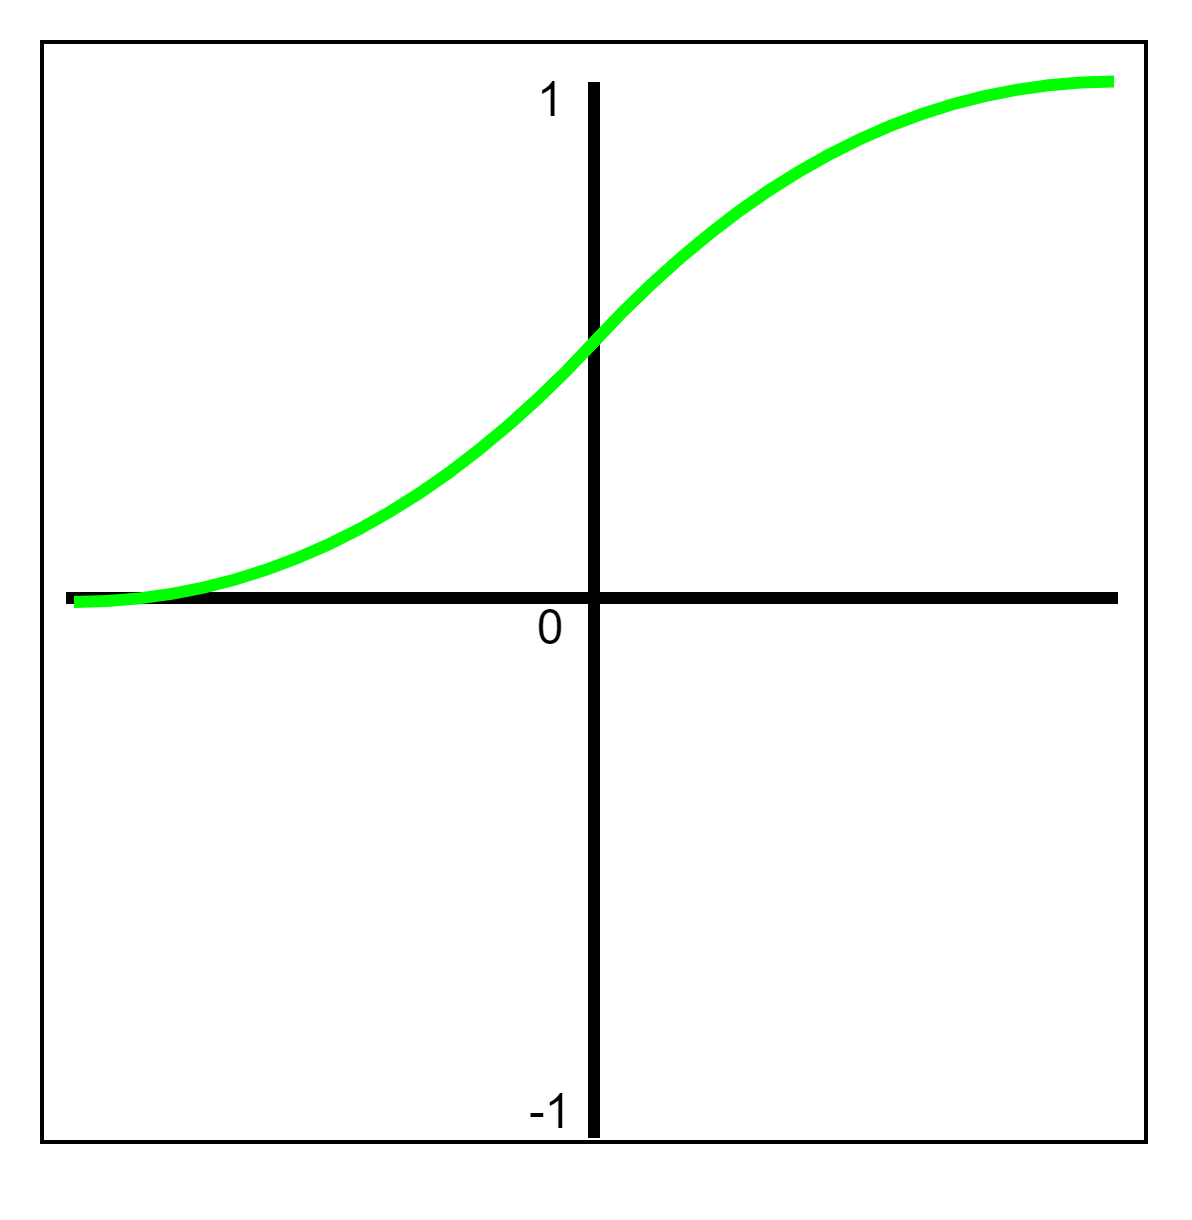
\includegraphics[width=0.4\linewidth]{figures/sigmoid_function.png}
\end{figure}
\end{frame}
%==========================================================================================
\begin{frame}
	\frametitle{Funções de Ativação}
	\begin{block}{Tanh}
		\begin{itemize}
			\item $y \in [-1, + 1]$
			\item Uma versão da Sigmoid
			\item Saída centrada em $0$
			\item Satura os gradientes. um pouco menos que a Sigmoid
			\item Converge lentamente
		\end{itemize}
		Função:
		$$f(x) = \frac{e^x - e^{-x}}{e^x+e^{-x}}$$
		Derivada: 	$$\frac{\partial y}{\partial x} = 1 - y^2$$
	\end{block}
\end{frame}
%==========================================================================================
\begin{frame}
	\frametitle{Funções de Ativação}
\begin{figure}
	\centering
	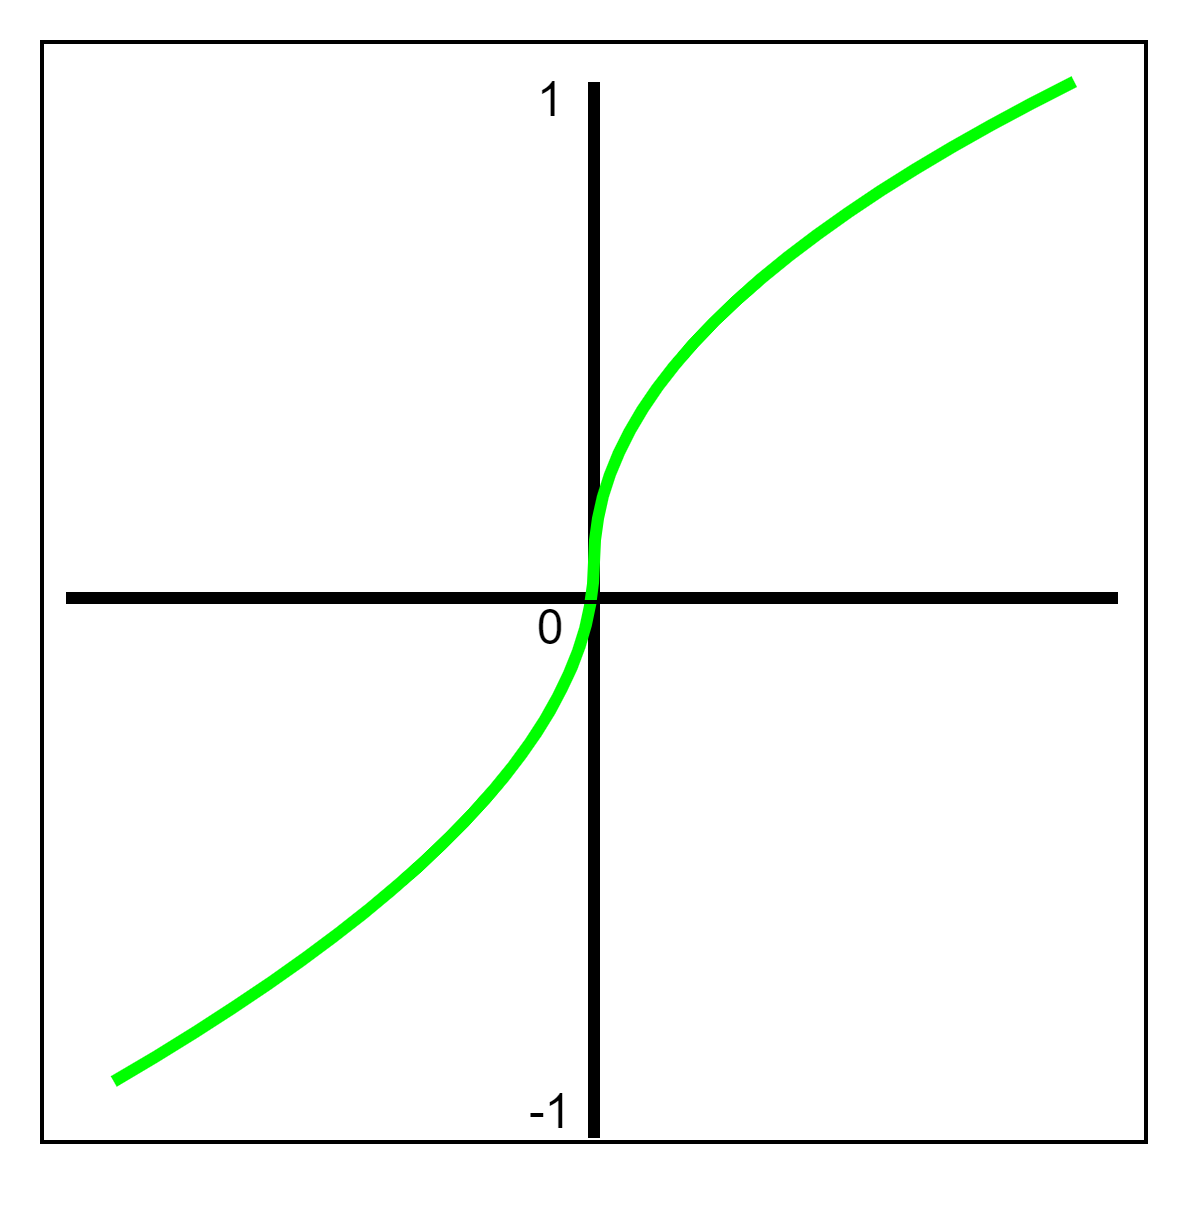
\includegraphics[width=0.4\linewidth]{figures/tanh_function}
\end{figure}
\end{frame}
%==========================================================================================
%==========================================================================================
\begin{frame}
	\frametitle{Funções de Ativação}
	\begin{block}{Relu}
		\begin{itemize}
			\item $y \in [0, + \infty]$
			\item Não tem derivada para valores $<0$
			\item Simples e Eficiente
			\item Evita a saturação dos gradientes
			\item Converge mais rápido
			\item Usada nas camadas escondidas
			\item Ela mata neurônio
		\end{itemize}
		Função:
		$$f(x) = max(0, x)$$
		Derivada: 	$$\frac{\partial y}{\partial x} =
		\left\{\begin{matrix}
			0,\; if \; x \leq 0
			\\ 
			1, \; if \; x > 0
		\end{matrix}\right.$$
	\end{block}
\end{frame}
%==========================================================================================
\begin{frame}
	\frametitle{Funções de Ativação}
	\begin{figure}
		\centering
		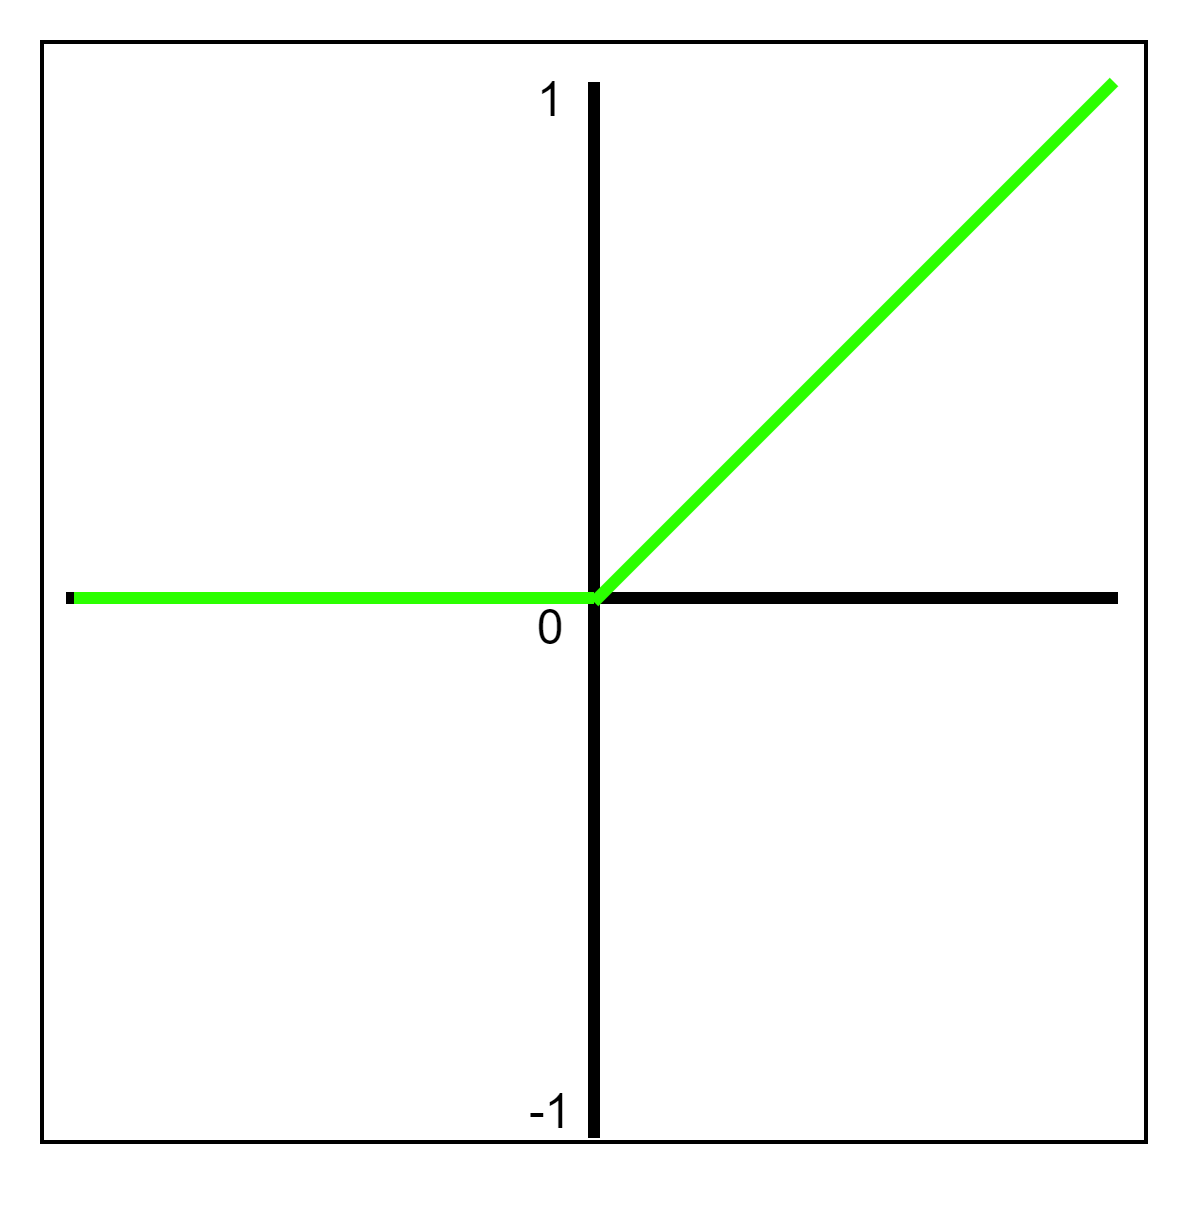
\includegraphics[width=0.4\linewidth]{figures/relu_function}
	\end{figure}
\end{frame}
%==========================================================================================
%==========================================================================================
\begin{frame}
	\frametitle{Funções de Ativação}
	\begin{block}{Leaky Relu}
		\begin{itemize}
			\item $y \in [- \infty, + \infty]$
			\item Tem derivada para valores $<0$
			\item Simples e Eficiente
			\item Evita a saturação dos gradientes
			\item Converge mais rápido
			\item Usada nas camadas escondidas
			\item Diminui as mortes de neurônios
		\end{itemize}
		Função:
		$$f(x) = 		\left\{\begin{matrix}
			\alpha(e^x - 1), x \leq 0
			\\ 
			x, x > 0
		\end{matrix}\right.$$
	
		Derivada: 	$$\frac{\partial y}{\partial x} =
		\left\{\begin{matrix}
			\alpha, x \leq 0
			\\ 
			1, x > 0
		\end{matrix}\right.$$
	\end{block}
\end{frame}
%==========================================================================================
\begin{frame}
	\frametitle{Funções de Ativação}
	\begin{figure}
		\centering
		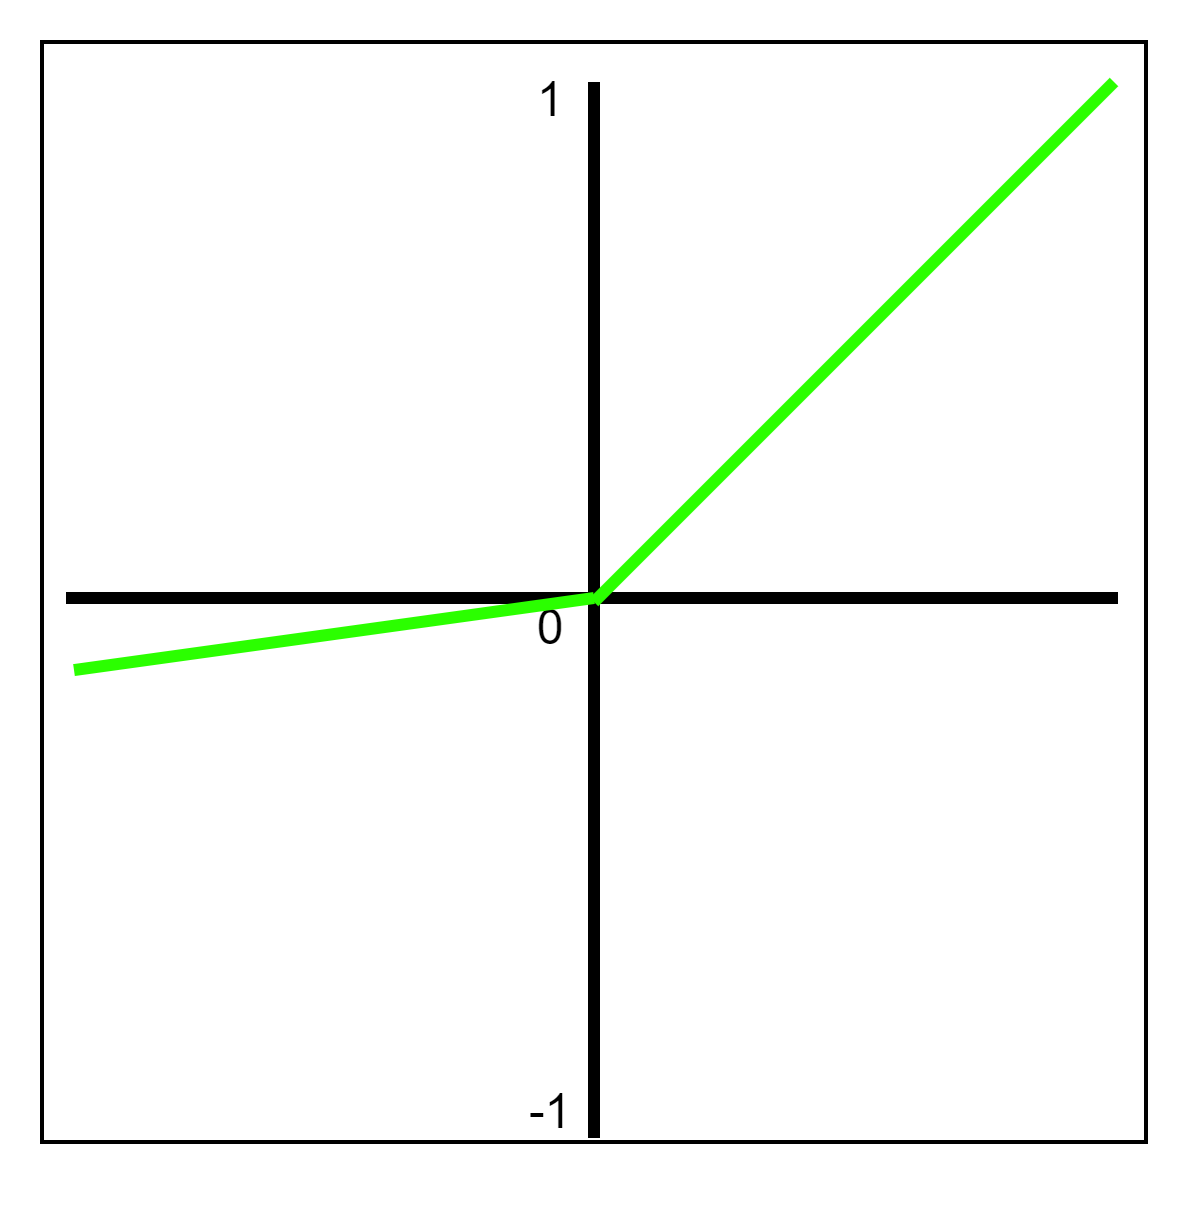
\includegraphics[width=0.4\linewidth]{figures/leaky_relu_function}
	\end{figure}
	
\end{frame}
%==========================================================================================
\begin{frame}
	\frametitle{Funções de Ativação}
	\begin{figure}
		\centering
		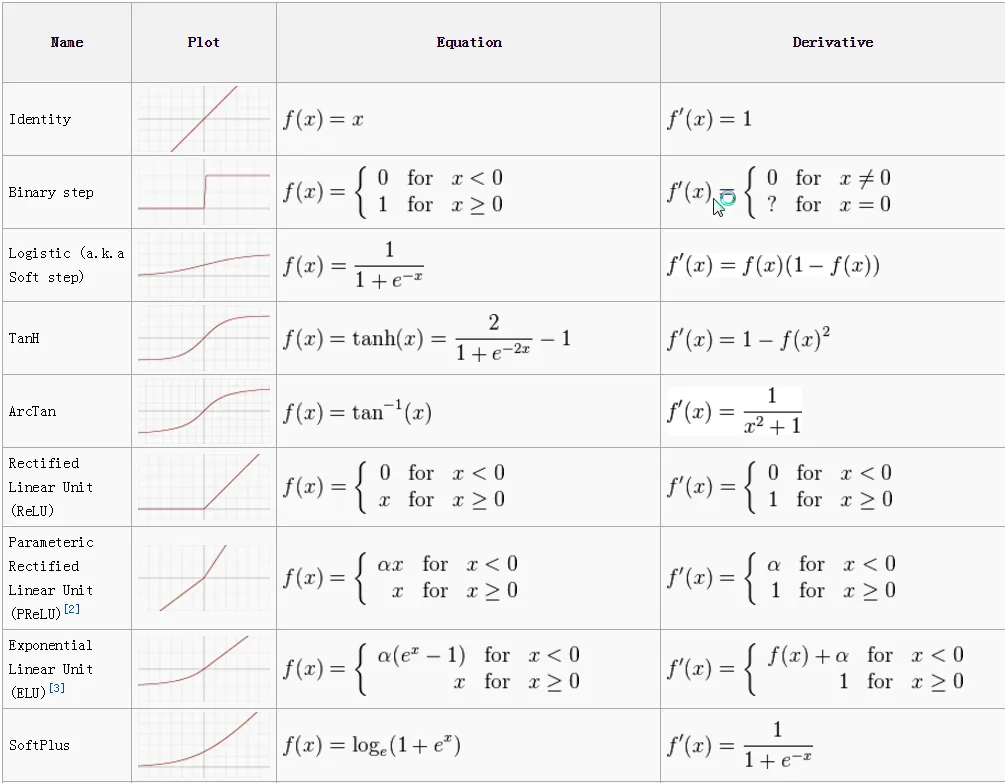
\includegraphics[width=0.7\linewidth]{figures/mais_activation_functions}
	\end{figure}

\end{frame}
%===================================================================================
%==========================================================================================
\begin{frame}
	\frametitle{Funções de Ativação}
	\begin{alertblock}{ Qual função de ativação usar?}
		\begin{itemize}
		\item	Evitar Sigmoid nas camadas ocultas, boa na saída
		\item	Tanh usada em modelos generativos
		\item	Relu Muito boa nas camadas ocultas
		\item	Linear não usar em camadas escondidas
		\item	Leaky Relu  raramente usadas
		\end{itemize}
	\end{alertblock}	
\end{frame}
%===================================================================================
\begin{frame}
	\frametitle{Funções de Ativação}
	\begin{block}{Softmax}
		\begin{itemize}
			\item $y \in [0, 1]$ e $\sum_y = 1$
			\item Aplicada em dois ou mais neurônios. Pega saída e converte
			\item A saída é uma confiança
			\item Nunca nas camadas ocultas
			\item Multiclasses
			\item Saída One-hot Encode
		\end{itemize}
		Função:
		$$S_i = \frac{e^{\hat{y}_i}}{\sum_j e^{\hat{y}_i}} $$
		Assim para cada k: $P^k = S_i^{[k]}$
		Derivada: 	$$\frac{\partial S}{\partial y} = p^k * (1-p^k)$$
	\end{block}
\end{frame}
%==========================================================================================
\begin{frame}
	\frametitle{Funções de Ativação}
	\begin{block}{Softmax}
		\begin{example}
			$[0.1, 1.3, 2.5] \to [0.07, 0.22, 0.72] $ \\
			$$\frac{e^{0.1}}{e^{0.1} + e^{0.3} + e^{2.5}}$$
		\end{example}
		Função:
		$$S_i = \frac{e^{\hat{y}_i}}{\sum_j e^{\hat{y}_i}} $$
		Assim para cada k: $P^k = S_i^{[k]}$
		Derivada: 	$$\frac{\partial y}{\partial x} =
		\left\{\begin{matrix}
			\alpha, x \leq 0
			\\ 
			1, x > 0
		\end{matrix}\right.$$
	\end{block}
\end{frame}
%==========================================================================================
%==========================================================================================
\begin{frame}
	\frametitle{Funções de Ativação}
	\begin{block}{Vamos ver na prática}
		Vamos praticar utilizando o notebook 03\_funções de ativação
	\end{block}
\end{frame}

%==========================================================================================
\section{Backpropagation}
\begin{frame}
	\frametitle{Backpropagation}
	\begin{block}{Para que usamos o \textit{backpropagation}?}
		Utilizamos o Backpropagation no treinamento das redes neurais
	\end{block}
	\begin{example}
		Vamos tomar uma função simples de multiplicação:
		$$f(x, y) = x * y$$
			
		\begin{figure}
			\centering
			
\includegraphics[width=0.5\linewidth]{figures/simple_multiply_gate}
		\end{figure}
	\end{example}
\end{frame}

%==========================================================================================
\begin{frame}
	\frametitle{Backpropagation}
	\begin{example}
		Vamos tomar uma função simples de multiplicação:
		$$f(x, y) = x * y$$
		
		\begin{figure}
			\centering
			
\includegraphics[width=0.5\linewidth]{figures/simple_multiply_gate_part1}
		\end{figure}
		\alert{Com que força alterar as entradas desse circuito para de maneira ``leve'' alteremos a saída?}
	\end{example}
\end{frame}
%==========================================================================================
\begin{frame}
	\frametitle{Backpropagation}
	\begin{example}
		Vamos tomar uma função simples de multiplicação:
		$$f(x, y) = x * y$$
		
\begin{figure}
	\centering
	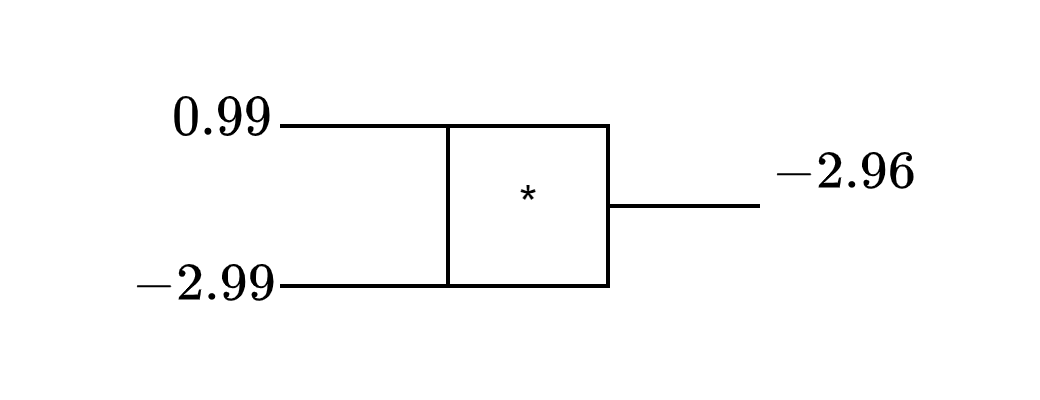
\includegraphics[width=0.5\linewidth]{figures/simple_multiply_gate_part2}
\end{figure}
		
	\end{example}
\end{frame}
%==========================================================================================
%==========================================================================================
%==========================================================================================
%==========================================================================================
%==========================================================================================
%==========================================================================================
%==========================================================================================
%==========================================================================================
%==========================================================================================
%==========================================================================================
%==========================================================================================
%==========================================================================================
%==========================================================================================
%==========================================================================================
%==========================================================================================
%==========================================================================================
%==========================================================================================
%==========================================================================================
%==========================================================================================
\section{Se Tornando Expert em Gradientes}

\begin{frame}
\frametitle{Highlighting text}

\begin{gather}
	W = np.random.randn(5, 10) \\
	X = np.random.randn(3, 10) \\
	Y = X.dot(W^{T}) \\
	f(x)
\end{gather}
%
%\begin{align}
%	a + b  q q= c \\        
%	a = c - b
%\end{align}
In this slide, some important text will be
\alert{highlighted} because it's important.
Please, don't abuse it.

\begin{block}{Remark}
Sample text
\end{block}

\begin{alertblock}{Important theorem}
Sample text in red box
\end{alertblock}

\begin{examples}
Sample text in green box. The title of the block is ``Examples".
\end{examples}
\end{frame}

\end{document}